\subsubsection{monolith::client::bubble::BaseBubble}

\label{monolith::client::bubble::BaseBubble}
\begin{figure}[H]
	\centering
	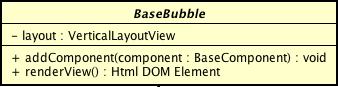
\includegraphics[scale=0.5]{Sezioni/SottosezioniST/img/BaseBubble.png}
	\caption{monolith::client::bubble::BaseBubble}
\end{figure}

\begin{itemize}
\item \textbf{Descrizione:} Classe base astratta che rappresenta le bolle di Monolith.
\item \textbf{Utilizzo:} Classe base astratta utilizzata ed estesa ogni qualvolta uno sviluppatore intende creare nuove bolle.
\item \textbf{Attributi:} 
\begin{itemize}
\item \textit{protected layout:VerticalLayoutView}\\
Oggetto che rappresenta il layout verticale di default della bolla.
\end{itemize}
\item \textbf{Metodi:}
\begin{itemize}
	\item \textit{public addComponent(component:BaseComponent):void}\\
Aggiunge un widget o layout alla bolla.
		  \\ \textbf{Parametri}: \begin{itemize}
				\item \textit{component:BaseComponent}\\
					Oggetto che rappresenta il componente che si desidera aggiungere alla bolla.
			\end{itemize}
	\item \textit{public getLayout():BaseLayout}\\
Questo metodo ritorna il layout principale della bolla.
	\item \textit{public renderView():HtmlDOMElement}\\
Restituisce l'elemento DOM rappresentante la bolla.
\end{itemize}
\end{itemize}

\subsubsection{monolith::client::bubble::ToDoListBubble}

\label{monolith::client::bubble::ToDoListBubble}
\begin{figure}[H]
	\centering
	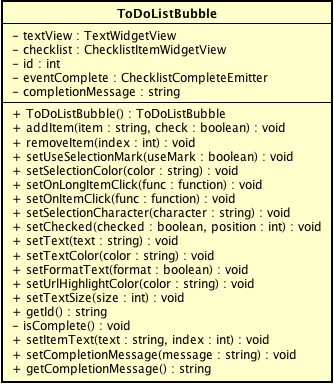
\includegraphics[scale=0.5]{Sezioni/SottosezioniST/img/ToDoListBubble.png}
	\caption{monolith::client::bubble::ToDoListBubble}
\end{figure}

\begin{itemize}
\item \textbf{Descrizione:} Classe concreta che estende BaseBubble, destinata alla creazione di bolle lista di Monolith.
\item \textbf{Utilizzo:} Classe utilizzata ogni qualvolta uno sviluppatore intende creare nuove bolle lista.
\item \textbf{Attributi:}
\begin{itemize}
\item \textit{private textView:TextWidgetView}\\
Oggetto che rappresenta il widget contenente il testo della bolla lista.
\item \textit{private checklist[]:ChecklistItemWidgetView}\\
Oggetto che rappresenta un'array contenente la lista di oggetti che si possono spuntare, sotto forma di widget di tipo ChecklistItem.
\item \textit {private id:string}\\
Stringa che rappresenta l'identificativo della bolla ToDo in questione.
\item \textit {private eventComplete:ChecklistCompleteEmitter}
Oggetto che permette di catturare gli eventi lanciati di tipo ChecklistComplete.
\item \textit {private completionMessage:string}
Stringa che viene visualizzata dalla bolla una volta spuntati tutti i suoi ChecklistItemWidget.
\end{itemize}
\item \textbf{Metodi:}
\begin{itemize}
\item \textit{private isComplete():void}\\
Questo metodo manda un evento di tipo ChecklistComplete quando tutti i ChecklistItemWidget della bolla in questione sono spuntati.
\item \textit{public ToDoListBubble():ToDoListBubble}\\
Il costruttore della classe ToDoListBubble.
\item \textit{public addItem(item:string,check:boolean):void}\\
Aggiunge un elemento con il nome definito alla bolla lista.
\\ \textbf{Parametri}: \begin{itemize}
\item \textit{item:string}\\
Valore che rappresenta il nome dell'elemento che si vuole aggiungere alla lista.
\item \textit{check:boolean}\\
Valore che rappresenta se la checkbox del ChecklistItemWidget che sta per essere aggiunto deve essere spuntata o no.
\end{itemize}
\item \textit{public removeItem{index:int}:void}\\
Permette di rimuovere un elemento dalla lista di oggetti di una bolla ToDo.
\\ \textbf{Parametri}: \begin{itemize}
\item \textit{index:int}\\
L'indice dell'elemento che si desidera rimuovere dall'array di di oggetti della bolla ToDo.
\item \textit{public setUseSelectionMark(useMark:boolean):void}\\
	Imposta la visualizzazione delle spunte con un carattere oppure con un colore.
		\\ \textbf{Parametri}: \begin{itemize}
		\item \textit{useMark:boolean}\\
		Se questo è a true la visualizzazione della spunta viene effettuata con un carattere, altrimenti la visualizzazione viene effettuata con un colore.
		\end{itemize}  
\item \textit{public setSelectionColor(color:string):void}\\
	Imposta il colore con il quale effettuare la visualizzazione delle spunte.
		\\ \textbf{Parametri}: \begin{itemize}
		\item \textit{color:string}\\
		Rappresenta la stringa in esadecimale corrispondente al colore che verrà impostato per visualizzare le spunte.
		\end{itemize}  
\item \textit{public setSelectionCharacter(character:string):void}\\
	Imposta il carattere utilizzato per la visualizzazione delle spunte.
		\\ \textbf{Parametri}: \begin{itemize}
		\item \textit{character:string}\\
		Il carattere utilizzato per la visualizzazione delle spunte.
		\end{itemize} 
\item \textit{public setChecked(checked:boolean,position:int):void}\\
	Permette di spuntare un oggetto della bolla ToDo o di togliere una spunta da esso.
		\\ \textbf{Parametri}: \begin{itemize}
		\item \textit{checked:boolean}\\
		Questo booleano è a true se si vorrà spuntare la entry, a false altrimenti.
		\item \textit{position:int}\\
		La posizione, all'interno della checklist, dell'elemento del quale si vuole modificare lo stato. 
		\end{itemize}
\item \textit{public setText(text:string):void}\\
	Imposta il testo all'interno del widget testo che rappresenta il titolo della bolla.
		\\ \textbf{Parametri}: \begin{itemize}
		\item \textit{text:string}\\
		Rappresenta con una string il testo che va inserito all'interno del widget.
		\end{itemize}
\item \textit{public setTextColor(color:string):void}\\
	Imposta il colore del testo del widget testo.
		\\ \textbf{Parametri}: \begin{itemize}
		\item \textit{color:string}\\
		Rappresenta la stringa in esadecimale corrispondente al colore che verrà come sfondo del bottone.
		\end{itemize}
\item \textit{public setFormatText(format: boolean):void}\\
	Imposta il widget a testo formattato o testo semplice.
		\\ \textbf{Parametri}: \begin{itemize}
		\item \textit{format: boolean}\\
		Questo booleano viene impostato a true se si vuole il testo del widget formattato, a false altrimenti.
		\end{itemize} 
\item \textit{public setUrlHighlightColor(color:boolean):void}\\
	Imposta la possibilità di cliccare o meno i link presenti nel testo del widget.
		\\ \textbf{Parametri}: \begin{itemize}
		\item \textit{color:string}\\
		Questo booleano viene impostato a true se si vogliono i link cliccabili, a false altrimenti.
		\end{itemize} 
\item \textit{public setTextSize(size:int):void}\\
	Imposta la grandezza del testo nel widget
		\\ \textbf{Parametri}: \begin{itemize}
		\item \textit{size:int}\\
		Rappresenta il numero di pixel corrispondente all'altezza del testo che verrà impostata all'interno del widget.
		\end{itemize}
\item \textit{public setOnItemClick(func:function):void}\\
	Imposta l'azione per il click normale della entry.
		\\ \textbf{Parametri}: \begin{itemize}
		\item \textit{func:function}\\
		La funzione che verrà impostata per il click normale della entry.
		\end{itemize} 
\item \textit{public setOnLongItemClick(func:function):void}\\
	Imposta l'azione per il click prolungato della entry.	
		\\ \textbf{Parametri}: \begin{itemize}
		\item \textit{func:function}\\
		La funzione che verrà impostata per il click prolungato della entry.
		\end{itemize}
\item \textit{public getId():string}\\
Restituisce l'identificativo della bolla.
\item \textit{public setItemText(text:string,index:int):void}\\
	Imposta il testo di uno specifico oggetto della bolla ToDo.
		\\ \textbf{Parametri}: \begin{itemize}
		\item \textit{text:string}\\
		Il testo che si vuole impostare all'interno dell'oggetto.
		\item \textit{index:int}\\
		L'indice corrispondente alla posizione del oggetto del quale si vuole impostare il testo.
		\end{itemize}
\item \textit{public setCompletionMessage(message:string):void}\\
Imposta il testo che la bolla ToDo visualizzerà una volta spuntati tutti i suoi oggetti.
	\\ \textbf{Parametri}: \begin{itemize}
		\item \textit{message:string}\\
		Il testo che la bolla ToDo visualizzerà una volta spuntati tutti i suoi oggetti.
	\end{itemize}
\item \textit{public getCompletionMessage():string}\\
Ritorna il testo che la bolla ToDo visualizzerà una volta spuntati tutti i suoi oggetti.

\end{itemize}
\end{itemize}
\end{itemize}

\subsubsection{monolith::client::bubble::MarkdownBubble}

\label{monolith::client::bubble::MarkdownBubble}
\begin{figure}[H]
	\centering
	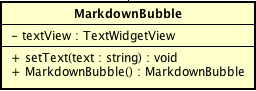
\includegraphics[scale=0.5]{Sezioni/SottosezioniST/img/MarkdownBubble.png}
	\caption{monolith::client::bubble::MarkdownBubble}
\end{figure}

\begin{itemize}
\item \textbf{Descrizione:} Classe concreta che estende BaseBubble, destinata alla creazione di bolle testo markdown di Monolith.
\item \textbf{Utilizzo:} Classe utilizzata ogni qualvolta uno sviluppatore intende creare nuove bolle testo markdown.
\item \textbf{Attributi:}
\begin{itemize}
\item \textit{private textview:TextWidgetView}\\
Oggetto che rappresenta il widget contenente il testo della bolla testo markdown.
\end{itemize}
\item \textbf{Metodi:}
\begin{itemize}
\item \textit{public MarkdownBubble():MarkdownBubble}\\
Il costruttore della classe MarkdownBubble.
\item \textit{public setText(text:string):void}\\
Imposta il testo della bolla con il valore definito.
\\ \textbf{Parametri}: \begin{itemize}
\item \textit{text:string}\\
Valore che rappresenta il testo che si vuole inserire nella bolla testo markdown.
\end{itemize}
\end{itemize}
\end{itemize}

\subsubsection{monolith::client::bubble::AlertBubble}

\label{monolith::client::bubble::AlertBubble}
\begin{figure}[H]
	\centering
	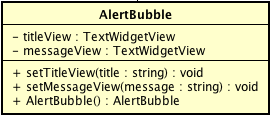
\includegraphics[scale=0.5]{Sezioni/SottosezioniST/img/AlertBubble.png}
	\caption{monolith::client::bubble::AlertBubble}
\end{figure}

\begin{itemize}
\item \textbf{Descrizione:} Classe concreta che estende BaseBubble, destinata alla creazione di bolle avviso di Monolith.
\item \textbf{Utilizzo:} Classe utilizzata ogni qualvolta uno sviluppatore intende creare nuove bolle avviso.
\item \textbf{Attributi:} 
\begin{itemize}
\item \textit{private titleView:TextWidgetView}\\
Campo che rappresenta e contiene il titolo della bolla avviso.
\item \textit{private messageView:TextWidgetView}\\
Campo che rappresenta e contiene il messaggio della bolla avviso.
\end{itemize}
\item \textbf{Metodi:}
\begin{itemize}
\item \textit{public AlertBubble():AlertBubble}\\
Il costruttore della classe AlertBubble.
\item \textit{public setTitle(title:string):void}\\
Imposta il titolo della bolla avviso con il valore title.
\\ \textbf{Parametri}: \begin{itemize}
\item \textit{title:string}\\
Valore che rappresenta il titolo che si vuole impostare alla bolla avviso.
\end{itemize}
\item \textit{public setMessage(message:string):void}\\
Imposta il messaggio della bolla avviso con il valore message.
\\ \textbf{Parametri}: \begin{itemize}
\item \textit{message:string}\\
Valore che rappresenta il messaggio testuale che si vuole impostare alla bolla avviso.
\end{itemize}
\end{itemize}
\end{itemize}